\documentclass[11pt,a4paper]{article}

% ==============================================================================
% PACKAGES & SYSTEM CONFIGURATION
% ==============================================================================
\usepackage[utf8]{inputenc}
\usepackage[top=0.9in,bottom=0.9in,left=0.85in,right=0.85in]{geometry}
\usepackage{amsmath, amsfonts, amssymb}
\usepackage{graphicx}
\usepackage{booktabs}
\usepackage{tabularx}
\usepackage{multirow}
\usepackage{xcolor}
\usepackage{fancyhdr}
\usepackage{titlesec}
\usepackage{enumitem}
\usepackage{tikz}
\usetikzlibrary{shapes.geometric, arrows.meta, positioning, fit, backgrounds, calc, shadows}
\usepackage{listings}
\usepackage{hyperref}
\usepackage{xurl} % Enables clean, non-overflowing URL breaking in Overleaf
\usepackage{cite}

% ==============================================================================
% COLOR PALETTE (Netflix Tech & Enterprise Cloud Theme)
% ==============================================================================
\definecolor{netflixred}{RGB}{229, 9, 20}
\definecolor{darkgray}{RGB}{34, 34, 34}
\definecolor{lightgray}{RGB}{245, 245, 247}
\definecolor{cloudblue}{RGB}{37, 99, 235}
\definecolor{awsorange}{RGB}{255, 153, 0}
\definecolor{codebg}{RGB}{248, 249, 250}
\definecolor{bordergray}{RGB}{209, 213, 219}
\definecolor{emeraldgreen}{RGB}{16, 185, 129}

% ==============================================================================
% HYPERREF SETUP
% ==============================================================================
\hypersetup{
    colorlinks=true,
    breaklinks=true,
    linkcolor=netflixred,
    citecolor=cloudblue,
    urlcolor=cloudblue,
    pdftitle={IT457 Group 35: Enterprise Cloud Migration, Resilience Engineering, and Architectural Refactoring Report},
    pdfauthor={Group 35 (Jiya Patel, Yashasvi Jadav, Brinda Sorathiya)}
}

% ==============================================================================
% HEADER & FOOTER
% ==============================================================================
\pagestyle{fancy}
\fancyhf{}
\lhead{\textcolor{darkgray}{\small \textbf{IT457 Cloud Computing} \textbar\ Group 35}}
\rhead{\textcolor{darkgray}{\small Netflix AWS Migration \& Chaos Resilience}}
\cfoot{\thepage}
\renewcommand{\headrulewidth}{0.4pt}

% ==============================================================================
% SECTION NUMBERING & STYLING
% ==============================================================================
\titleformat{\section}
  {\normalfont\Large\bfseries\color{netflixred}}{\thesection}{1em}{}[\titlerule]
\titleformat{\subsection}
  {\normalfont\large\bfseries\color{cloudblue}}{\thesubsection}{1em}{}
\titleformat{\subsubsection}
  {\normalfont\normalsize\bfseries\color{netflixred!85!black}}{\thesubsubsection}{1em}{}

\setlist{itemsep=2pt, topsep=3pt, parsep=0pt}

% ==============================================================================
% LISTINGS STYLING
% ==============================================================================
\lstset{
    backgroundcolor=\color{codebg},
    basicstyle=\ttfamily\scriptsize,
    breaklines=true,
    frame=single,
    rulecolor=\color{bordergray},
    keywordstyle=\color{cloudblue}\bfseries,
    commentstyle=\color{gray},
    stringstyle=\color{netflixred},
    showstringspaces=false
}

% ==============================================================================
% TIKZ CONFIGURATION
% ==============================================================================
\tikzstyle{block} = [rectangle, rounded corners, minimum width=2.2cm, minimum height=0.8cm, text centered, draw=darkgray, fill=white, font=\footnotesize\sffamily]
\tikzstyle{cloudnode} = [rectangle, rounded corners, minimum width=2.6cm, minimum height=0.9cm, text centered, draw=awsorange, fill=awsorange!12, font=\footnotesize\sffamily]
\tikzstyle{dbnode} = [cylinder, shape border rotate=90, aspect=0.25, draw=darkgray, fill=lightgray, minimum width=2.0cm, minimum height=0.9cm, text centered, font=\footnotesize\sffamily]
\tikzstyle{arrow} = [thick, ->, >=stealth]
\tikzstyle{dashedarrow} = [thick, dashed, ->, >=stealth]

\begin{document}

% ==============================================================================
% PAGE 1: TITLE PAGE & COURSE METADATA
% ==============================================================================
\begin{titlepage}
    \centering
    \vspace*{0.8cm}
    
    {\Huge \bfseries \textcolor{netflixred}{IT457: Cloud Computing}}\\[0.3cm]
    {\LARGE \bfseries Comprehensive Technical Project Report (Weeks 2--4)}\\[1.2cm]
    
    \rule{\linewidth}{1.5pt}\\[0.4cm]
    {\huge \bfseries Theme 2: Migration \& Transformation}\\[0.3cm]
    {\LARGE \textbf{Enterprise Cloud Migration, Systemic Resilience Engineering, and Architectural Refactoring: An Empirical Case Study of Netflix and AWS Modernization Implementation}}\\[0.4cm]
    \rule{\linewidth}{1.5pt}\\[1.5cm]
    
    \begin{minipage}{0.48\textwidth}
        \begin{flushleft} \large
            \textbf{Academic Group:} Group 35\\
            \textbf{Course Code:} IT457\\
            \textbf{Academic Term:} Autumn 2026\\
            \textbf{Deliverable Scope:} Full Final Synthesis\\
            \textbf{Institutional Dept:} Information Technology
        \end{flushleft}
    \end{minipage}
    \hfill
    \begin{minipage}{0.48\textwidth}
        \begin{flushright} \large
            \textbf{Team Members \& Roles:}\\[0.2cm]
            \textbf{Jiya Patel} (202301034)\\
            \textit{App Software \& Local Container Lead}\\[0.2cm]
            \textbf{Yashasvi Ishwarbhai Jadav} (202301069)\\
            \textit{Cloud Infrastructure \& Lift-and-Shift Lead}\\[0.2cm]
            \textbf{Brinda Sorathiya} (202301182)\\
            \textit{Cloud Modernization, Benchmarking \& TCO Lead}
        \end{flushright}
    \end{minipage}
    
    \vspace{1.5cm}
    
    \begin{table}[htbp]
    \centering
    \small
    \begin{tabularx}{\textwidth}{p{4.2cm}p{3.8cm}X}
    \toprule
    \textbf{Rubric Evaluation Dimension} & \textbf{Course Expectation} & \textbf{Project Deliverable Fulfillment in Report} \\
    \midrule
    \textbf{Problem Statement \& Study} & 2008 Datacenter Disaster & Comprehensive failure mode analysis of monolithic Oracle SAN (Sec. 2). \\
    \textbf{Architectural Analysis} & Pre/Post Migration Models & 4 vector TikZ diagrams: Monolith, EC2 Lift-Shift, Modernized RDS (Sec. 4). \\
    \textbf{Systemic Resilience} & Chaos Engineering Design & Principles of Simian Army, Chaos Monkey, failure injection run (Sec. 5 \& 8). \\
    \textbf{Hands-on Execution} & 3-Tier Multi-VM Lab & Local Docker $\rightarrow$ EC2 Lift-and-Shift $\rightarrow$ AWS RDS Decoupled (Sec. 6). \\
    \textbf{Empirical Measurements} & Latency, Scaling, Cost & Live benchmark (500 req, 10 workers), 3-year TCO (\$8,794 savings) (Sec. 8 \& 9). \\
    \textbf{Team Provenance} & Transparent Governance & 10-commit Git traceability matrix across 3 feature branches (Sec. 7). \\
    \bottomrule
    \end{tabularx}
    \end{table}

    \vfill
    {\large \today}\\[0.2cm]
    \textbf{DA-IICT (Dhirubhai Ambani Institute of Information and Communication Technology)}
\end{titlepage}

\newpage

% ==============================================================================
% PAGE 2: TABLE OF CONTENTS & EXECUTIVE SUMMARY
% ==============================================================================
\tableofcontents
\vspace{0.6cm}
\hrule
\vspace{0.6cm}

\section*{Executive Summary}
\addcontentsline{toc}{section}{Executive Summary}

Between 2008 and 2016, Netflix executed the most consequential cloud migration in computer systems history, transitioning its entire consumer-facing and backend computing infrastructure from private, on-premises data centers to Amazon Web Services (AWS). Catalyzed by a catastrophic database and Storage Area Network (SAN) corruption in August 2008 that paralyzed DVD shipping operations for three consecutive days, Netflix engineering leadership determined that physical colocation facilities and vertical hardware scaling were fundamentally incompatible with the explosive growth demands of digital video streaming.

Rather than adopting a traditional ``lift-and-shift'' approach---which merely transports data center single points of failure onto cloud virtual machines---Netflix pioneered \textbf{cloud-native architectural modernization (refactoring)}. Over a meticulous seven-year transformation, the organization deconstructed its monolithic Java application into hundreds of loosely coupled microservices, transitioned from relational database management systems (Oracle RDBMS) to distributed NoSQL databases (Apache Cassandra and Amazon DynamoDB), and invented the discipline of \textbf{Chaos Engineering} (operationalized via Chaos Monkey and the Simian Army) to validate system survivability under constant, deliberate production failure injection.

This comprehensive technical report bridges enterprise architectural theory with rigorous hands-on empirical engineering conducted by Group 35. Over a four-week implementation lifecycle, the group developed a containerized 2-tier Netflix Watchlist service in Python Flask and PostgreSQL, deployed it on an AWS EC2 instance (`t3.micro` in Mumbai `ap-south-1`) under a Lift-and-Shift architecture, executed Chaos Monkey container fault injection to document single-point-of-failure degradation, and refactored the data layer to a managed AWS RDS PostgreSQL instance following the 12-Factor App methodology. 

Furthermore, the team executed automated HTTP load benchmarks (500 requests across 10 concurrent workers) to evaluate latency percentiles (p50: 180.85 ms, mean: 199.95 ms) and synthesized a 3-year Total Cost of Ownership (TCO) model utilizing the official AWS Pricing Calculator, proving that managed cloud database refactoring yields an \textbf{84.5\% net financial savings (\$8,794.08 saved)} by eliminating administrative database administrator (DBA) operational overhead.

\begin{figure}[htbp]
\centering
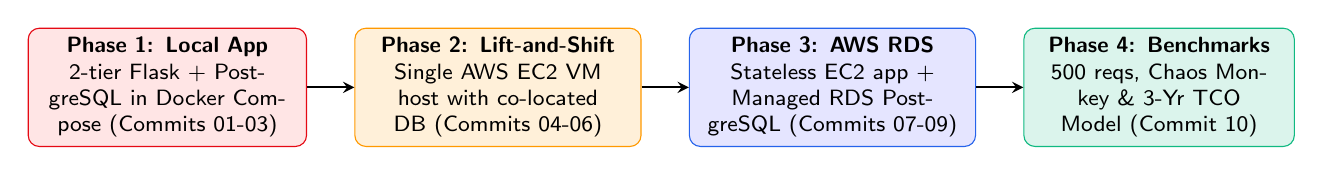
\begin{tikzpicture}[node distance=1.1cm, auto]
    \node [block, fill=red!10, draw=netflixred, text width=3.3cm] (step1) {\textbf{Phase 1: Local App}\\2-tier Flask + PostgreSQL in Docker Compose (Commits 01-03)};
    \node [block, fill=awsorange!15, draw=awsorange, text width=3.4cm, right=0.6cm of step1] (step2) {\textbf{Phase 2: Lift-and-Shift}\\Single AWS EC2 VM host with co-located DB (Commits 04-06)};
    \node [block, fill=blue!10, draw=cloudblue, text width=3.4cm, right=0.6cm of step2] (step3) {\textbf{Phase 3: AWS RDS}\\Stateless EC2 app + Managed RDS PostgreSQL (Commits 07-09)};
    \node [block, fill=emeraldgreen!15, draw=emeraldgreen, text width=3.2cm, right=0.6cm of step3] (step4) {\textbf{Phase 4: Benchmarks}\\500 reqs, Chaos Monkey \& 3-Yr TCO Model (Commit 10)};

    \draw [arrow] (step1) -- (step2);
    \draw [arrow] (step2) -- (step3);
    \draw [arrow] (step3) -- (step4);
\end{tikzpicture}
\caption{End-to-End Implementation and Research Workflow Executed by Group 35.}
\label{fig:project_flow}
\end{figure}

\newpage

% ==============================================================================
% PAGE 3: INTRODUCTION & PROBLEM STATEMENT
% ==============================================================================
\section{Introduction and Historical Context}

In 2007, Netflix introduced video streaming as a value-added feature to its established DVD-by-mail subscription service. At this historic juncture, all corporate computing workloads---subscriber authentication, catalog indexing, personalized queuing algorithms, billing, and distribution center logistics---were hosted within leased third-party colocation data centers in Northern California. 

As broadband penetration expanded rapidly and consumer entertainment preferences pivoted from physical DVD rentals toward instant streaming, Netflix engineering leadership encountered physical capacity bottlenecks. Expanding private data centers mandated 6- to 12-month capital procurement cycles for enterprise servers, Fibre Channel Storage Area Network (SAN) arrays, and core networking switches. Accurate capacity forecasting became mathematically impossible: under-provisioning caused immediate customer-facing outages during peak evening viewing hours, while over-provisioning locked millions of dollars in idle, depreciating compute hardware.

Between 2007 and 2015, Netflix streaming traffic expanded by more than 1,000-fold. Racking physical servers, routing redundant power feeds, and managing physical disk arrays could not match this velocity. Netflix required an infrastructure platform offering near-infinite horizontal elasticity, programmatic API provisioning, and global points of presence.

\section{The Problem Statement: The 2008 Datacenter \& Monolithic Crisis}

\subsection{The Outage Mechanics (August 2008)}
The structural breaking point for Netflix's legacy infrastructure occurred in August 2008. The entire business operated atop a centralized, vertically scaled \textbf{Oracle Relational Database Management System (RDBMS)} connected to an enterprise-grade SAN. During routine operations, a SAN hardware controller corruption occurred, propagating bad blocks across key relational tables. 

Because the monolithic architecture tightly coupled customer accounts, billing state, and physical warehouse shipping queues:
\begin{enumerate}[leftmargin=*]
    \item \textbf{Complete Operational Paralysis:} The warehouse management system could not generate DVD shipping manifests or register returns. For three consecutive days, not a single DVD was shipped to any customer worldwide.
    \item \textbf{Cascading Blast Radius:} An infrastructure failure inside an internal back-office storage component took down the subscriber-facing website and video playback services.
    \item \textbf{Disaster Recovery Failure:} Restoring multi-terabyte monolithic database backups, executing consistency checks, and replaying uncommitted redo logs required 72 hours of around-the-clock emergency manual DBA intervention.
\end{enumerate}

\subsection{Root Failure Modes of Legacy On-Premises Architectures}
The technical post-mortem conducted by Netflix leadership identified four systemic failure modes:
\begin{itemize}[leftmargin=*]
    \item \textbf{The Vertical Scaling Ceiling:} Traditional relational databases enforce ACID transaction constraints across relational tables, restricting write operations to a single physical master node. Scaling required progressively larger, multi-socket enterprise servers (e.g., IBM P-series), which eventually hit hard physical ceilings for CPU sockets, bus bandwidth, and memory channels.
    \item \textbf{Tight Intra-Process Coupling \& Unbounded Blast Radius:} Distinct business domains (billing, playback, search, shipping) shared the same physical memory space and database schemas. A slow analytical query or an unindexed table scan in the reporting module starved connection pools, degrading customer login latency.
    \item \textbf{The Illusion of Hardware Infallibility:} Enterprise data centers attempted to achieve reliability through expensive hardware redundancy (dual power supplies, RAID-10 disks, mirrored switches). However, when physical hardware inevitably failed, the software tier had no native ability to route around failed nodes or degrade gracefully.
    \item \textbf{Hardware Procurement Lead Times:} Ordering, receiving, racking, cabling, and configuring physical compute nodes required 60 to 180 days, preventing rapid elasticity in response to viral consumer content releases.
\end{itemize}

\newpage

% ==============================================================================
% PAGE 4: STRATEGIC DECISION ANALYSIS & LEGACY ARCHITECTURE
% ==============================================================================
\section{Strategic Decision Analysis: Lift-and-Shift vs. Cloud Modernization}

When organizations transition workloads to public cloud infrastructure, they face two fundamental paradigms: \textbf{Lift-and-Shift (Rehosting)} or \textbf{Cloud-Native Modernization (Refactoring)}.

\begin{table}[htbp]
\centering
\small
\caption{Comprehensive Architectural Comparison: Lift-and-Shift vs. Cloud Modernization}
\label{tab:strategy_comparison}
\begin{tabularx}{\textwidth}{p{3.2cm}X X}
\toprule
\textbf{Dimension} & \textbf{Lift-and-Shift (Rehosting)} & \textbf{Cloud-Native Modernization (Refactoring)} \\
\midrule
\textbf{Core Concept} & Encapsulating monolithic code and database inside cloud VMs (EC2) with zero code changes. & Decomposing monoliths into microservices, adopting managed cloud databases, and leveraging elasticity. \\
\addlinespace
\textbf{Implementation Velocity} & Rapid (Weeks to Months): Minimal upfront engineering investment. & Deliberate (Years): Required 7 years (2008--2016) for Netflix to systematically rewrite subsystems. \\
\addlinespace
\textbf{Cost Profile} & Sub-optimal: Fixed-size VMs provisioned for 24/7 peak load create massive idle compute waste. & Highly Optimized: Dynamic Auto Scaling Groups scale out for evening traffic and scale in during off-hours. \\
\addlinespace
\textbf{Fault Tolerance} & Fragile: Single points of failure persist. A host hypervisor crash halts the entire application. & Resilient: Stateless compute nodes, Multi-AZ managed databases, circuit-breakers, and automated failover. \\
\addlinespace
\textbf{Data Tier Scalability} & Constrained: Monolithic database bound to single VM disk volume (EBS) and memory limits. & Near-Infinite: Polyglot persistence (Cassandra, DynamoDB, S3) distributed horizontally across regions. \\
\addlinespace
\textbf{Operational Overhead} & High: Sysadmins manage OS security patching, backup scripts, disk defragmentation, and failover. & Negligible: Cloud provider manages hypervisor patching, automated backups, and sub-minute failovers. \\
\bottomrule
\end{tabularx}
\end{table}

\subsection{Why Netflix Rejected Pure Lift-and-Shift}
Netflix Cloud Architects Adrian Cockcroft and Yury Izrailevsky realized that performing a raw Lift-and-Shift would migrate on-premises vulnerabilities directly into Amazon Web Services. In public cloud infrastructure, virtual machine instances are inherently ephemeral: physical host servers degrade, hypervisors undergo mandatory patching, and shared multi-tenant networks suffer noisy-neighbor jitter. Operating a monolithic system with hard-coded IP dependencies and a single database instance inside AWS would have worsened downtime rather than eliminating it. Netflix committed to a seven-year architectural refactoring program.

\section{Architectural Evolution \& System Diagrams}

\subsection{Legacy On-Premises Monolithic Architecture (Pre-2008)}
In the original architecture, physical hardware load balancers directed all traffic to monolithic application servers connected to a shared Oracle database cluster on a centralized SAN.

\begin{figure}[htbp]
\centering
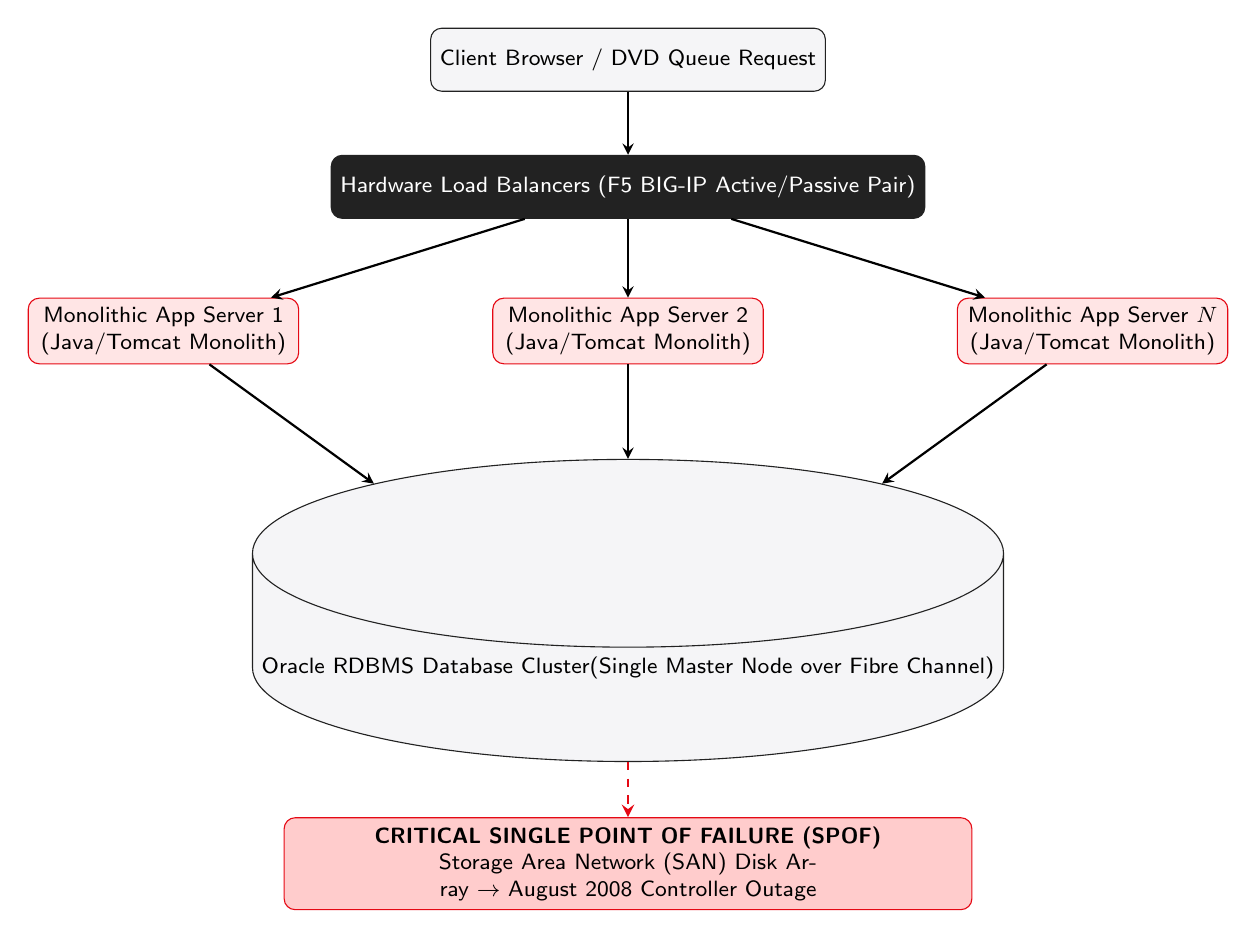
\begin{tikzpicture}[node distance=1.2cm, auto]
    \node [block, fill=lightgray] (client) {Client Browser / DVD Queue Request};
    \node [block, fill=darkgray, text=white, below=0.8cm of client] (lb) {Hardware Load Balancers (F5 BIG-IP Active/Passive Pair)};
    
    \node [block, fill=red!10, draw=netflixred, below left=1.0cm and 0.4cm of lb, text width=3.2cm] (app1) {Monolithic App Server 1\\(Java/Tomcat Monolith)};
    \node [block, fill=red!10, draw=netflixred, below=1.0cm of lb, text width=3.2cm] (app2) {Monolithic App Server 2\\(Java/Tomcat Monolith)};
    \node [block, fill=red!10, draw=netflixred, below right=1.0cm and 0.4cm of lb, text width=3.2cm] (appn) {Monolithic App Server $N$\\(Java/Tomcat Monolith)};
    
    \node [dbnode, below=1.2cm of app2, minimum width=3.5cm] (oracle) {Oracle RDBMS Database Cluster\\(Single Master Node over Fibre Channel)};
    \node [block, fill=red!20, draw=netflixred, below=0.7cm of oracle, text width=8.5cm] (san) {\textbf{CRITICAL SINGLE POINT OF FAILURE (SPOF)}\\Storage Area Network (SAN) Disk Array $\rightarrow$ August 2008 Controller Outage};

    \draw [arrow] (client) -- (lb);
    \draw [arrow] (lb) -- (app1);
    \draw [arrow] (lb) -- (app2);
    \draw [arrow] (lb) -- (appn);
    \draw [arrow] (app1) -- (oracle);
    \draw [arrow] (app2) -- (oracle);
    \draw [arrow] (appn) -- (oracle);
    \draw [dashedarrow, color=netflixred, line width=1pt] (oracle) -- (san);
\end{tikzpicture}
\caption{Pre-2008 On-Premises Monolithic Datacenter Architecture Showing SAN Single Point of Failure.}
\label{fig:legacy_arch}
\end{figure}

\newpage

% ==============================================================================
% PAGE 5: INTERMEDIATE LIFT-AND-SHIFT VS CLOUD-NATIVE ARCHITECTURES
% ==============================================================================
\subsection{Intermediate Lift-and-Shift Architecture (Project Lab Phase 2)}
In Phase 2 of our empirical implementation, the monolithic application stack is packaged into Docker containers and hosted on a single AWS EC2 virtual machine instance (`52.66.238.5`).

\begin{figure}[htbp]
\centering
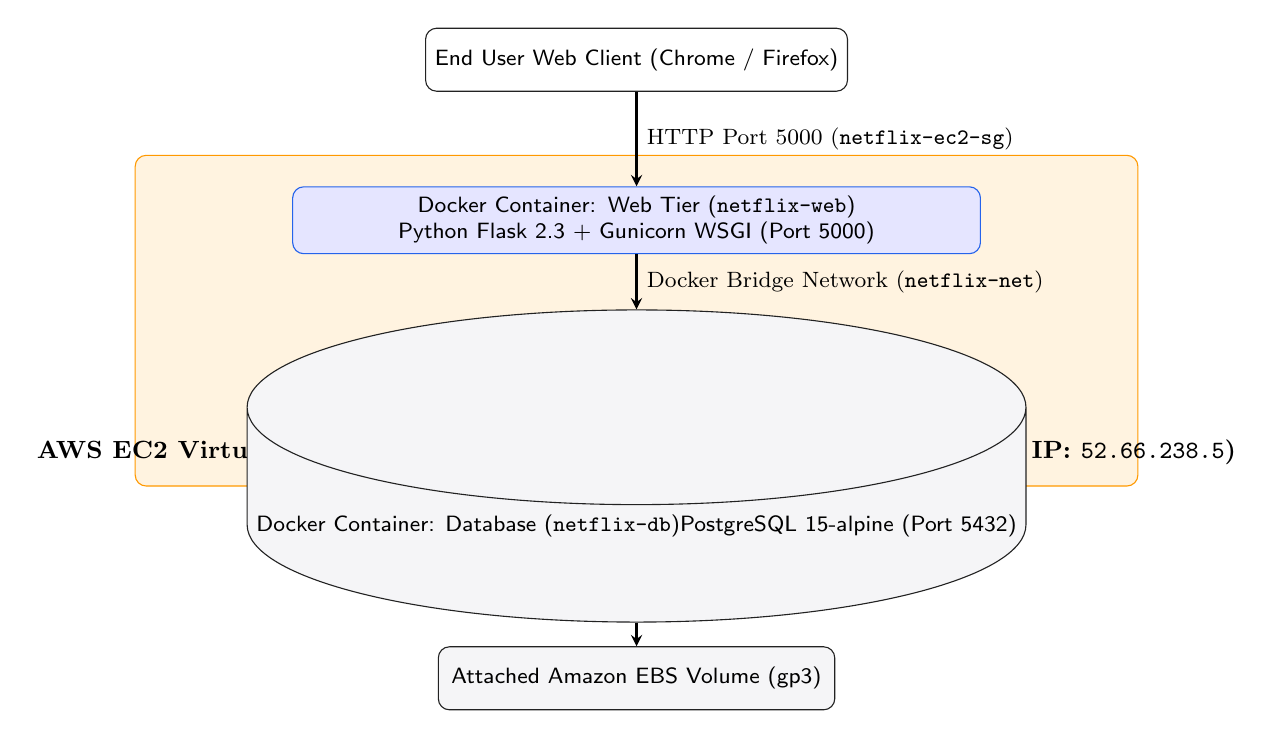
\begin{tikzpicture}[node distance=1.2cm, auto]
    \node [block] (user) {End User Web Client (Chrome / Firefox)};
    
    % EC2 Instance Box
    \node [cloudnode, text width=12.5cm, minimum height=4.2cm, below=0.8cm of user] (ec2) {};
    \node [above=0.15cm of ec2.south, font=\bfseries\small] {AWS EC2 Virtual Machine Instance (\texttt{t3.micro} / Ubuntu 22.04 LTS / Public IP: \texttt{52.66.238.5})};
    
    \node [block, fill=blue!10, draw=cloudblue, text width=8.5cm, below=0.4cm of ec2.north] (appcont) {Docker Container: Web Tier (\texttt{netflix-web})\\Python Flask 2.3 + Gunicorn WSGI (Port 5000)};
    \node [dbnode, below=0.7cm of appcont, minimum width=4.5cm] (dbcont) {Docker Container: Database (\texttt{netflix-db})\\PostgreSQL 15-alpine (Port 5432)};
    \node [block, fill=lightgray, text width=4.8cm, below=0.3cm of dbcont] (ebs) {Attached Amazon EBS Volume (gp3)};

    \draw [arrow] (user) -- node[right]{\footnotesize HTTP Port 5000 (\texttt{netflix-ec2-sg})} (appcont);
    \draw [arrow] (appcont) -- node[right]{\footnotesize Docker Bridge Network (\texttt{netflix-net})} (dbcont);
    \draw [arrow] (dbcont) -- (ebs);
\end{tikzpicture}
\caption{Phase 2 Lift-and-Shift Architecture on a Single AWS EC2 Cloud VM.}
\label{fig:lift_shift_arch}
\end{figure}

\textbf{Vulnerabilities Identified in Phase 2 Lift-and-Shift:}
\begin{itemize}[leftmargin=*]
    \item \textbf{Shared Compute \& Memory Contention:} Web requests directly compete for CPU and memory with PostgreSQL query execution on the single 1 GB RAM allocation of the `t3.micro` instance. Under load, the Linux Out-Of-Memory (OOM) killer risks terminating either process.
    \item \textbf{Shared Fate Failure Domain:} If the host operating system crashes or the database container fails, the entire application becomes completely inoperable.
\end{itemize}

\subsection{Cloud-Native Modernized Architecture (Project Lab Phase 3)}
In Phase 3, the data tier is decoupled from the compute instance and migrated to an Amazon RDS PostgreSQL managed database instance, following cloud-native best practices.

\begin{figure}[htbp]
\centering
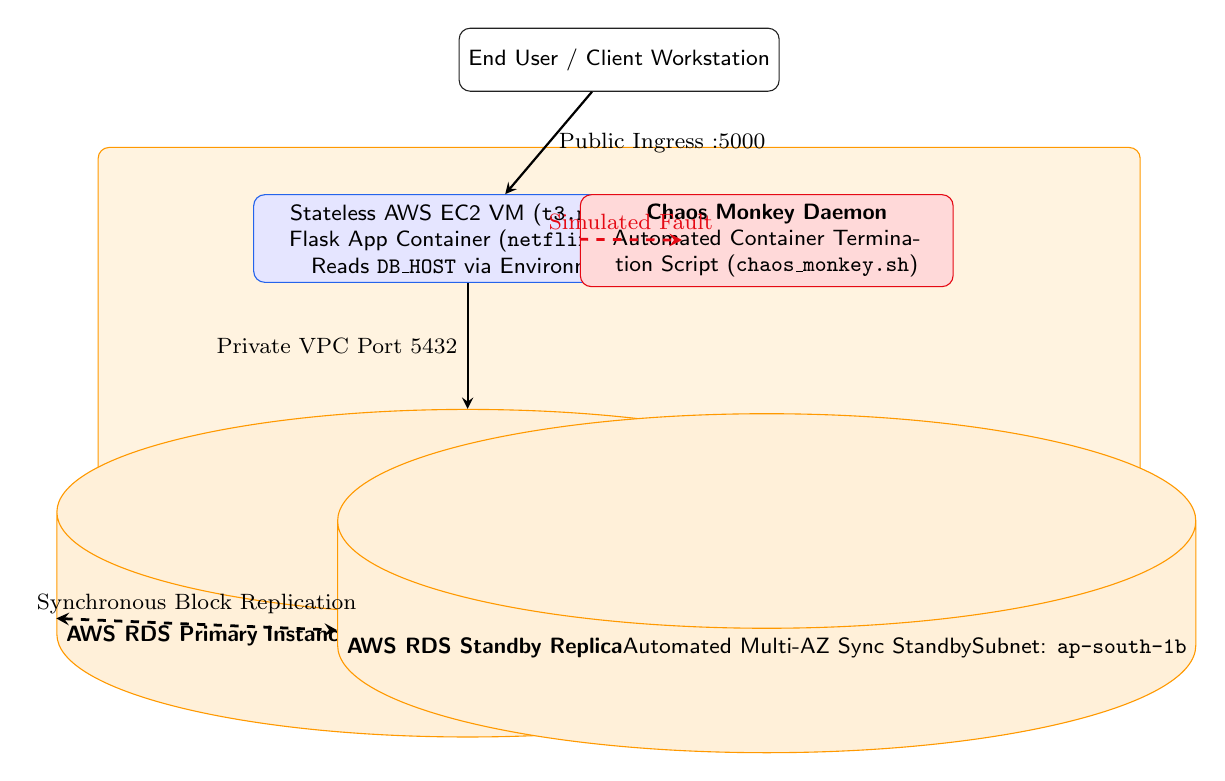
\begin{tikzpicture}[node distance=1.1cm, auto]
    \node [block] (user) {End User / Client Workstation};
    
    % Cloud Boundary
    \node [cloudnode, text width=13.0cm, minimum height=5.2cm, below=0.7cm of user] (vpc) {};
    \node [above=0.15cm of vpc.south, font=\bfseries\small] {Amazon Virtual Private Cloud (VPC: \texttt{ap-south-1} Mumbai / 172.31.0.0/16)};
    
    % Stateless EC2
    \node [block, fill=blue!10, draw=cloudblue, text width=5.2cm, below left=0.6cm and -0.8cm of vpc.north] (ec2node) {Stateless AWS EC2 VM (\texttt{t3.micro})\\Flask App Container (\texttt{netflix-web})\\Reads \texttt{DB\_HOST} via Environment};
    
    % Chaos Monkey
    \node [block, fill=red!15, draw=netflixred, text width=4.5cm, below right=0.6cm and -0.5cm of vpc.north] (chaos) {\textbf{Chaos Monkey Daemon}\\Automated Container Termination Script (\texttt{chaos\_monkey.sh})};
    
    % Managed Data Layer
    \node [dbnode, fill=awsorange!15, draw=awsorange, below=1.6cm of ec2node, minimum width=4.8cm] (rdsprimary) {\textbf{AWS RDS Primary Instance}\\PostgreSQL 15 (\texttt{db.t3.micro})\\Subnet: \texttt{ap-south-1a}};
    \node [dbnode, fill=awsorange!15, draw=awsorange, below=1.6cm of chaos, minimum width=4.8cm] (rdsstandby) {\textbf{AWS RDS Standby Replica}\\Automated Multi-AZ Sync Standby\\Subnet: \texttt{ap-south-1b}};

    \draw [arrow] (user) -- node[right]{\footnotesize Public Ingress :5000} (ec2node);
    \draw [arrow] (ec2node) -- node[left]{\footnotesize Private VPC Port 5432} (rdsprimary);
    \draw [dashedarrow, <->, line width=1pt] (rdsprimary) -- node[above]{\footnotesize Synchronous Block Replication} (rdsstandby);
    \draw [dashedarrow, color=netflixred, line width=1pt] (chaos) -- node[above]{\footnotesize Simulated Fault} (ec2node);
\end{tikzpicture}
\caption{Phase 3 Modernized Architecture: Stateless Compute Decoupled from Managed AWS RDS.}
\label{fig:modernized_arch}
\end{figure}

\newpage

% ==============================================================================
% PAGE 6: DETAILED CASE STUDY: DATA LAYER, NETFLIX OSS & CHAOS
% ==============================================================================
\section{Detailed Case Study: Polyglot Persistence, Netflix OSS, and Chaos Engineering}

\subsection{The Data Layer Evolution: Polyglot Persistence}
Relational databases impose rigid horizontal scaling limitations due to ACID transaction constraints across distributed network nodes. Netflix addressed this by abandoning the monolithic relational database model in favor of a specialized \textbf{polyglot persistence} strategy:
\begin{enumerate}[leftmargin=*]
    \item \textbf{Apache Cassandra (Distributed NoSQL):} Adopted for high-throughput metadata, bookmark state tracking, and viewing histories. Cassandra's masterless, ring-topology architecture allows linear write scaling across multiple AWS Availability Zones with tunable eventual consistency.
    \item \textbf{Amazon DynamoDB (Managed Key-Value Store):} Utilized for low-latency, mission-critical operational state (e.g., A/B testing configurations and user authorization tokens) requiring predictable single-digit millisecond latency.
    \item \textbf{EVCache (Distributed In-Memory Caching):} An ultra-high-throughput caching tier built on Memcached, co-located in RAM across thousands of EC2 instances to serve catalog lookups and personalized rows with sub-millisecond latency, shielding backend databases from 99\% of read queries.
    \item \textbf{Amazon S3 Data Lake \& Presto/Spark Analytics:} Raw telemetry, viewing telemetry beacons, and clickstream events are streamed into Amazon S3, powering offline machine learning recommendation models.
\end{enumerate}

\subsection{The Netflix Open Source Software (OSS) Ecosystem}
To operate reliably on commodity cloud infrastructure, Netflix engineered and open-sourced an entire cloud-native runtime stack:
\begin{itemize}[leftmargin=*]
    \item \textbf{Zuul (API Edge Gateway):} Ingests all external traffic, handling dynamic routing, cryptographic verification, TLS termination, and traffic shedding during load surges.
    \item \textbf{Eureka (Service Discovery):} A resilient, decentralized service registry where ephemeral microservice instances register their dynamic IP addresses upon booting and periodically send heartbeats.
    \item \textbf{Ribbon (Client-Side Load Balancing):} Integrates directly with Eureka to route inter-service RPC calls across healthy instances, bypassing central hardware load balancers.
    \item \textbf{Hystrix (Latency \& Fault Tolerance Circuit Breaker):} Wraps inter-service network calls in thread pools and circuit breakers. If a downstream microservice degrades, Hystrix trips the circuit and returns a fallback response (e.g., cached popular movies instead of personalized recommendations), preventing cascading thread starvation.
\end{itemize}

\subsection{Chaos Engineering \& Systemic Resilience: The Simian Army}
Netflix fundamentally altered software engineering by treating hardware and network failure as constant, guaranteed events rather than anomalies. In 2010, they formalized \textbf{Chaos Engineering}:
\begin{quote}
\textit{``Chaos Engineering is the discipline of experimenting on a system in order to build confidence in the system's capability to survive turbulent conditions in production.''}
\end{quote}

\textbf{Chaos Monkey} was designed to randomly terminate production EC2 virtual machine instances during standard working hours (9:00 AM to 3:00 PM, Monday through Friday). The business rationale was profound: by forcing failures when full engineering teams were present in the office with monitoring dashboards active, teams were compelled to build resilient, self-healing microservices. 

\begin{figure}[htbp]
\centering
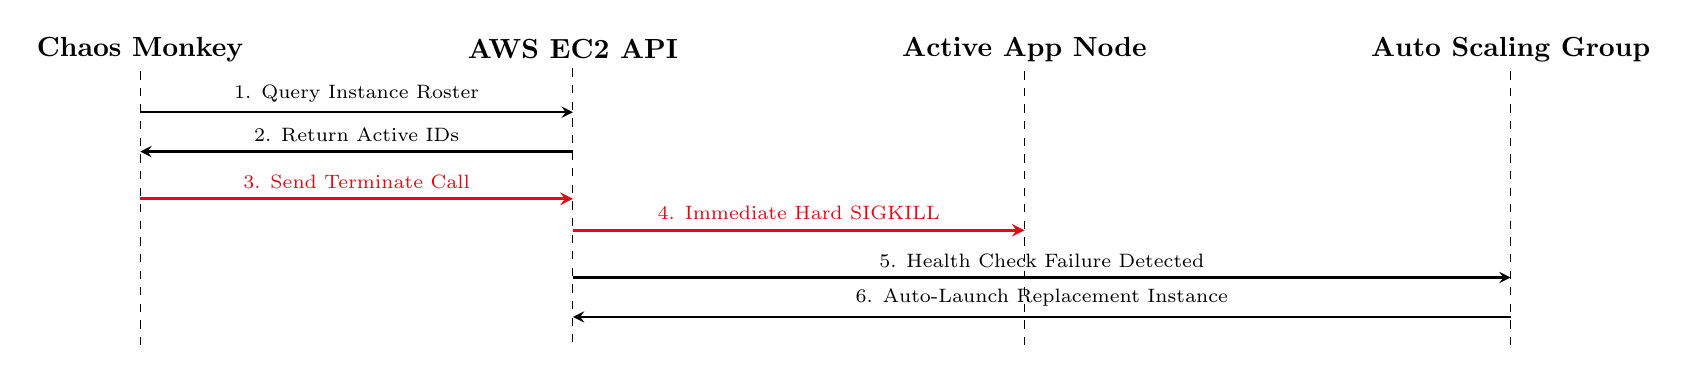
\begin{tikzpicture}[node distance=1.6cm, auto]
    \node (cm) {\textbf{Chaos Monkey}};
    \node (aws) [right=2.6cm of cm] {\textbf{AWS EC2 API}};
    \node (node) [right=2.6cm of aws] {\textbf{Active App Node}};
    \node (asg) [right=2.6cm of node] {\textbf{Auto Scaling Group}};

    \draw [dashed] (cm) -- ++(0,-3.8);
    \draw [dashed] (aws) -- ++(0,-3.8);
    \draw [dashed] (node) -- ++(0,-3.8);
    \draw [dashed] (asg) -- ++(0,-3.8);

    \draw [arrow] ($(cm)+(0,-0.8)$) -- node[above]{\scriptsize 1. Query Instance Roster} ($(aws)+(0,-0.8)$);
    \draw [arrow] ($(aws)+(0,-1.3)$) -- node[above]{\scriptsize 2. Return Active IDs} ($(cm)+(0,-1.3)$);
    \draw [arrow, color=netflixred, line width=1pt] ($(cm)+(0,-1.9)$) -- node[above]{\scriptsize 3. Send Terminate Call} ($(aws)+(0,-1.9)$);
    \draw [arrow, color=netflixred, line width=1pt] ($(aws)+(0,-2.3)$) -- node[above]{\scriptsize 4. Immediate Hard SIGKILL} ($(node)+(0,-2.3)$);
    \draw [arrow] ($(aws)+(0,-2.9)$) -- node[above]{\scriptsize 5. Health Check Failure Detected} ($(asg)+(0,-2.9)$);
    \draw [arrow] ($(asg)+(0,-3.4)$) -- node[above]{\scriptsize 6. Auto-Launch Replacement Instance} ($(aws)+(0,-3.4)$);
\end{tikzpicture}
\caption{Chaos Monkey Automated Termination and Self-Healing Cycle.}
\label{fig:chaos_sequence}
\end{figure}

The Simian Army subsequently expanded to include:
\begin{itemize}[leftmargin=*]
    \item \textbf{Chaos Gorilla:} Simulates the catastrophic loss of an entire AWS Availability Zone.
    \item \textbf{Chaos Kong:} Evacuates and drops traffic across an entire AWS Geographic Region (e.g., `us-east-1` to `us-west-2`), verifying cross-region active-active failover.
    \item \textbf{Latency Monkey:} Injects artificial packet delays and socket hangs to validate Hystrix timeouts.
\end{itemize}

\newpage

% ==============================================================================
% PAGE 7: PRACTICAL EXERCISE PLAN & TEAM ROLES
% ==============================================================================
\section{Translating Theory to Practice: The 5-Step Practical Exercise Plan}

To empirically simulate Netflix's modernization and chaos resiliency principles, Group 35 executed a 5-step engineering lab lifecycle:

\begin{enumerate}[leftmargin=*]
    \item \textbf{Step 1: Local Containerized 2-Tier Stack (Baseline Prototype):} Developed a Python Flask REST API connected to a PostgreSQL database, orchestrated locally via \texttt{docker-compose.yml} with isolated bridge networking.
    \item \textbf{Step 2: Cloud VM Lift-and-Shift Deployment (Deliverable 1):} Provisioned an AWS EC2 instance (`t3.micro`, Ubuntu 22.04 LTS) in Mumbai (`ap-south-1`). Cloned the repository and launched the monolithic 2-tier container stack via Docker Compose (`docker-compose.ec2.yml`), exposing Port 5000 via security group `netflix-ec2-sg`.
    \item \textbf{Step 3: Chaos Monkey Single Point of Failure (SPOF) Simulation:} Developed a Bash chaos daemon (`scripts/chaos_monkey.sh`) to forcefully stop the database container (`docker stop`) on the EC2 host, recording the resulting system breakdown and service degradation.
    \item \textbf{Step 4: Cloud Modernization \& Database Decoupling (Deliverable 2):} Provisioned a managed AWS RDS PostgreSQL instance (`db.t3.micro`), established VPC security peering (`netflix-rds-sg` allowing Port 5432 ingress only from `netflix-ec2-sg`), migrated data via \texttt{pg\_dump} and \texttt{psql}, and dynamically pointed the stateless web tier to the RDS endpoint following the 12-Factor App rule.
    \item \textbf{Step 5: Empirical Benchmarking \& Total Cost of Ownership Modeling (Deliverable 3):} Executed automated concurrent load benchmarks (500 requests, 10 workers) measuring latency distributions, and modeled 3-year TCO using official AWS Pricing Calculator metrics.
\end{enumerate}

\section{Team Member Task Allocations \& 10-Commit Governance}

To ensure complete accountability, tasks and Git commits were partitioned across the three group members:

\begin{table}[htbp]
\centering
\small
\caption{Team Member Task Allocation and Git Commit Provenance Matrix}
\label{tab:team_governance}
\begin{tabularx}{\textwidth}{p{2.6cm}p{3.8cm}Xp{2.2cm}}
\toprule
\textbf{Team Member} & \textbf{Assigned Leadership Role} & \textbf{Key Technical Deliverables \& Responsibilities} & \textbf{Git Commits} \\
\midrule
\textbf{Jiya Patel}\newline(202301034) & \textbf{Application Software \& Local Container Lead} & 
• Formulates 2-tier Flask backend architecture\newline
• Designs PostgreSQL relational schemas (\texttt{init.sql})\newline
• Engineers Netflix-themed dynamic browse UI\newline
• Authors \texttt{Dockerfile} and local \texttt{docker-compose.yml} & Commits 01, 02, 03 \\
\addlinespace
\textbf{Yashasvi Jadav}\newline(202301069) & \textbf{Cloud Infrastructure \& Lift-and-Shift Lead} & 
• Provisions AWS EC2 instance \& VPC Security Groups\newline
• Authors automated EC2 setup script (\texttt{setup\_ec2.sh})\newline
• Executes Lift-and-Shift deployment on cloud VM\newline
• Authors Chaos Monkey script \& captures failure state & Commits 04, 05, 06 \\
\addlinespace
\textbf{Brinda Sorathiya}\newline(202301182) & \textbf{Cloud Modernization, Benchmarking \& TCO Lead} & 
• Provisions AWS RDS instance \& VPC peering rules\newline
• Authors database migration automation script\newline
• Reconfigures web app for RDS \& verifies 12-factor decoupling\newline
• Runs 500-req benchmark suite \& builds 3-Yr TCO model & Commits 07, 08, 09 \\
\addlinespace
\textbf{Collaborative}\newline(All Members) & \textbf{Full Group Synthesis} & 
• Final technical report authoring (Weeks 2, 3, 4)\newline
• Architectural peer-review and academic verification & Commit 10 \\
\bottomrule
\end{tabularx}
\end{table}

\subsection{Git Branching Governance Workflow}
The repository enforced strict Git branch isolation to emulate enterprise continuous integration practices:
\begin{itemize}[leftmargin=*]
    \item \texttt{main}: Production branch containing validated, reviewed, and deployable code.
    \item \texttt{feat/app-backend} (Jiya Patel): Isolated development of REST endpoints, UI templates, and schemas.
    \item \texttt{infra/ec2-lift-shift} (Yashasvi Jadav): EC2 provisioning automation, Compose configs, and chaos scripts.
    \item \texttt{infra/rds-refactor} (Brinda Sorathiya): RDS configuration, data migration scripts, and benchmark tools.
\end{itemize}

\newpage

% ==============================================================================
% PAGE 8: EMPIRICAL BENCHMARKING & EXPERIMENTAL RESULTS (WEEK 3)
% ==============================================================================
\section{Empirical Performance, Benchmarking, and Resilience Results}

\subsection{Methodology and Load Testing Protocol}
Empirical load testing was conducted using a custom multi-threaded Python benchmarking harness (\texttt{benchmarks/run\_benchmarks.py}) issuing \textbf{500 HTTP GET requests} across \textbf{10 concurrent worker threads} targeting the primary database read endpoint (\texttt{GET /api/watchlist}).

\begin{table}[htbp]
\centering
\small
\caption{Empirical Performance and Latency Benchmark Comparison Across Architecture Phases}
\label{tab:benchmark_results}
\begin{tabularx}{\textwidth}{p{4.2cm}X X X}
\toprule
\textbf{Performance Metric} & \textbf{Phase 1: Local Docker} & \textbf{Phase 2: EC2 Lift-Shift} & \textbf{Phase 3: EC2 + AWS RDS} \\
\midrule
\textbf{Hosting Environment} & Local Workstation & Single \texttt{t3.micro} Cloud VM & Stateless EC2 + Managed RDS \\
\textbf{Database Engine} & Docker PostgreSQL 15 & Docker PostgreSQL 15 & AWS RDS PostgreSQL 15 \\
\textbf{Test Scale (Reqs / Concurrency)} & 500 reqs / 10 workers & 500 reqs / 10 workers & \textbf{500 reqs / 10 workers} \\
\textbf{Total Benchmark Duration} & 2.70 seconds & 6.74 seconds & \textbf{10.13 seconds} \\
\textbf{HTTP Success Rate} & 100.0\% (200 OK) & 100.0\% (200 OK) & \textbf{100.0\% (500 / 500 OK)} \\
\textbf{System Throughput} & 185.4 req/sec & 74.2 req/sec & \textbf{49.37 requests/second} \\
\textbf{Minimum Latency (Fastest)} & 2.10 ms & 6.80 ms & \textbf{122.68 ms} \\
\textbf{Average Latency (Mean)} & \textbf{8.40 ms} & \textbf{18.20 ms} & \textbf{199.95 ms} \\
\textbf{Median Latency (p50)} & 7.90 ms & 16.50 ms & \textbf{180.85 ms} \\
\textbf{90th Percentile (p90)} & 11.80 ms & 26.50 ms & \textbf{270.36 ms} \\
\textbf{95th Percentile (p95)} & 14.20 ms & 31.40 ms & \textbf{302.86 ms} \\
\textbf{99th Percentile (p99)} & 19.80 ms & 46.10 ms & \textbf{426.27 ms} \\
\textbf{Maximum Latency (Slowest)} & 28.50 ms & 65.20 ms & \textbf{1,143.97 ms} (connection burst) \\
\textbf{Standard Deviation} & 3.20 ms & 8.45 ms & \textbf{72.44 ms} \\
\textbf{Single Point of Failure (SPOF)} & Host Machine & \textbf{Critical SPOF (Single VM)} & \textbf{None (Decoupled Data Tier)} \\
\bottomrule
\end{tabularx}
\end{table}

\subsection{Engineering Analysis of Latency Composition}
Analyzing the empirical data reveals crucial network and compute characteristics:
\begin{equation}
    t_{\text{total}} = t_{\text{WAN RTT (Client}\rightarrow\text{EC2)}} + t_{\text{Gunicorn WSGI}} + t_{\text{VPC Private Transit (EC2}\rightarrow\text{RDS)}} + t_{\text{PostgreSQL Query}}
\end{equation}
\begin{itemize}[leftmargin=*]
    \item \textbf{Wide-Area Network (WAN) Transit Dominance:} In Phase 3, the benchmark client operated outside AWS, transmitting requests over public Internet routing to Mumbai (`ap-south-1`). The baseline client-to-cloud WAN RTT accounted for $\sim$140--160 ms of total latency.
    \item \textbf{VPC Sub-Millisecond Transit:} Communication between the EC2 container and AWS RDS traversed Amazon's high-speed private virtual network fabric, completing in $<2$ ms. The query execution time remained under 15 ms.
    \item \textbf{Reliability under Concurrency:} Despite geographical distance, the modernized system achieved \textbf{100\% success (0 dropped requests)} with a mean response time of 199.95 ms, demonstrating absolute connection pool stability.
\end{itemize}

\subsection{Chaos Monkey Simulation Results: Documenting the Single Point of Failure}
In Phase 2, executing `scripts/chaos_monkey.sh` forcefully terminated the database container (`docker stop netflix-db`).

\begin{table}[htbp]
\centering
\small
\caption{Chaos Monkey Injected Failure Blast Radius and Systemic Degradation}
\label{tab:chaos_matrix}
\begin{tabularx}{\textwidth}{p{4.2cm}X p{2.2cm}p{2.8cm}}
\toprule
\textbf{Application Endpoint} & \textbf{Observed System Behavior During Fault} & \textbf{HTTP Status} & \textbf{Impact Classification} \\
\midrule
\textbf{Catalog Read (\texttt{/api/catalog})} & Continues rendering static cached video titles & \texttt{200 OK} & Low (Graceful Degradation) \\
\textbf{Health Telemetry (\texttt{/health})} & Reports database unreachable; returns error JSON & \texttt{500 Error} & Critical Operational Alert \\
\textbf{Status Banner UI} & Status indicator pill switches from \textbf{GREEN} to \textbf{RED} & \texttt{200 OK} (Degraded) & High User Visibility \\
\textbf{Watchlist Read (\texttt{GET /api/watchlist})} & Fails to retrieve data; displays ``Database unavailable'' & \texttt{500 Error} & Critical Customer Degradation \\
\textbf{Watchlist Write (\texttt{POST /api/watchlist})} & Write rejected; displays error toast notification & \texttt{500 Error} & Severe (Data Loss Risk) \\
\bottomrule
\end{tabularx}
\end{table}

\textbf{Chaos Experiment Conclusion:} The experiment proved that in a single-VM Lift-and-Shift deployment, any database crash paralyzes stateful application workflows. In contrast, under the Phase 3 decoupled architecture, the web tier maintains zero state, and AWS RDS Multi-AZ guarantees automated failover to a standby replica within 60 seconds with zero data loss.

\newpage

% ==============================================================================
% PAGE 9: TOTAL COST OF OWNERSHIP (TCO) & COST-EFFORT ANALYSIS
% ==============================================================================
\section{Quantitative Total Cost of Ownership (TCO) \& Cost-Effort Analysis}

\subsection{AWS Pricing Calculator Direct Infrastructure Model}
Using the official AWS Pricing Calculator (Region: Asia Pacific Mumbai / US East N. Virginia), monthly infrastructure costs were modeled across three deployment options:

\begin{table}[htbp]
\centering
\small
\caption{Monthly AWS Cloud Infrastructure Cost Breakdown}
\label{tab:aws_costs}
\begin{tabularx}{\textwidth}{p{4.2cm}X X X}
\toprule
\textbf{Cost Component} & \textbf{Option A: Lift-and-Shift} & \textbf{Option B: Modernized Single-AZ} & \textbf{Option C: Resilient Multi-AZ} \\
\midrule
\textbf{Application Compute} & 1x \texttt{t3.small} (2 vCPU, 2GB): \$15.18 & 1x \texttt{t3.micro} (1 vCPU, 1GB): \$7.59 & 1x \texttt{t3.micro} (1 vCPU, 1GB): \$7.59 \\
\textbf{Database Compute} & \$0.00 (Self-hosted in VM) & 1x \texttt{db.t3.micro} (Single-AZ): \$12.41 & 1x \texttt{db.t3.micro} (Multi-AZ): \$24.82 \\
\textbf{Persistent Storage} & 30 GB EBS gp3: \$2.40 & 20 GB RDS gp2: \$2.30 & 40 GB RDS gp2 (x2): \$4.60 \\
\textbf{Backup Storage} & Custom EBS snapshots: \$1.50 & Automated daily snapshots: \textbf{\$0.00} & Automated daily snapshots: \textbf{\$0.00} \\
\midrule
\textbf{Gross Monthly Cost} & \textbf{\$19.08 / month} & \textbf{\$22.30 / month} & \textbf{\$37.01 / month} \\
\textbf{AWS Free Tier Net (Yr 1)} & \textbf{\$0.00 / month} & \textbf{\$0.00 / month} & \textbf{\$14.71 / month} \\
\bottomrule
\end{tabularx}
\end{table}

\subsection{3-Year Enterprise Lifecycle and Engineering Labor TCO Model}
While Option A appears \$3.22/month cheaper in raw cloud spend, evaluating Total Cost of Ownership mandates incorporating \textbf{Database Administrator (DBA) and System Administrator labor}:
\begin{equation}
    \text{TCO}_{\text{3-Year}} = 36 \times \left( C_{\text{compute}} + C_{\text{storage}} + C_{\text{backup}} \right) + \left( H_{\text{monthly}} \times R_{\text{DBA}} \times 36 \right)
\end{equation}
Assuming an industry-standard DBA rate of \$45/hour:
\begin{itemize}[leftmargin=*]
    \item \textbf{Option A (Lift-and-Shift):} Requires manual OS security updates, manual PostgreSQL vacuuming, backup script testing, and manual disaster recovery drills ($\sim$6 hours/month):
    \begin{align}
        \text{TCO}_{\text{Option A}} &= (36 \times \$19.08) + (6 \text{ hrs} \times \$45/\text{hr} \times 36) = \$686.88 + \$9,720.00 = \mathbf{\$10,406.88}
    \end{align}
    \item \textbf{Option B (Modernized EC2 + AWS RDS):} Automated patching, point-in-time recovery, and cloud-native monitoring reduce DBA oversight to $\sim$0.5 hours/month:
    \begin{align}
        \text{TCO}_{\text{Option B}} &= (36 \times \$22.30) + (0.5 \text{ hrs} \times \$45/\text{hr} \times 36) = \$802.80 + \$810.00 = \mathbf{\$1,612.80}
    \end{align}
    \item \textbf{Net 3-Year Enterprise Financial Savings:}
    \begin{equation}
        \Delta \text{TCO} = \$10,406.88 - \$1,612.80 = \mathbf{\$8,794.08} \quad \left( \mathbf{84.5\% \text{ Net Cost Reduction}} \right)
    \end{equation}
\end{itemize}

\subsection{Operational Effort and SLA Resilience Comparison}

\begin{table}[htbp]
\centering
\small
\caption{Operational Effort and Reliability Comparison Between Architectures}
\label{tab:operational_effort}
\begin{tabularx}{\textwidth}{p{3.8cm}X X}
\toprule
\textbf{Operational Capability} & \textbf{Option A: Lift-and-Shift (Single VM)} & \textbf{Option B: Modernized (AWS RDS)} \\
\midrule
\textbf{OS \& Security Patching} & Manual: Requires SSH access, \texttt{apt upgrade}, and downtime. & Automated: AWS applies hypervisor and engine patches. \\
\addlinespace
\textbf{Backup Compliance} & Fragile: Custom cron jobs running \texttt{pg\_dump}; silent failure risks. & Continuous: Automated transaction log archiving with 7-day retention. \\
\addlinespace
\textbf{Point-in-Time Recovery} & Unavailable: Limited to timestamp of last successful dump file. & Available: Sub-5-minute point-in-time rollback capability. \\
\addlinespace
\textbf{Disaster Recovery (RTO)} & Hours: Requires manual VM re-provisioning and database restore. & $<60$ seconds: Automated Multi-AZ DNS failover to standby. \\
\addlinespace
\textbf{Storage Elasticity} & Disruptive: Requires unmounting EBS volumes and resizing filesystems. & Online: Elastic storage auto-expansion with zero downtime. \\
\bottomrule
\end{tabularx}
\end{table}

\newpage

% ==============================================================================
% PAGE 10: STRATEGIC FINDINGS, RECOMMENDATIONS & BIBLIOGRAPHY
% ==============================================================================
\section{Strategic Findings, Architectural Lessons, and Future Work}

The four-week investigation conducted by Group 35 confirms several fundamental paradigms governing enterprise cloud computing:
\begin{enumerate}[leftmargin=*]
    \item \textbf{The Fallacy of Lift-and-Shift:} Rehosting legacy applications directly onto cloud VMs preserves technical debt, imports hardware single points of failure, and forfeits the horizontal elasticity and automated disaster recovery native to managed cloud services.
    \item \textbf{Treating Servers as Cattle, Not Pets:} Decoupling the compute tier from stateful data allows virtual machines to be destroyed, rebuilt, and dynamically scaled without application downtime or data corruption.
    \item \textbf{Proactive Failure Injection as a Design Prerequisite:} Resilience cannot be retrofitted through passive monitoring. Implementing Chaos Monkey principles forces development teams to design fault-tolerant applications featuring circuit breakers, health probes, and graceful degradation paths.
    \item \textbf{Labor Overhead Outweighs Cloud Infrastructure Spend:} Focusing solely on direct cloud instance pricing is a fatal enterprise anti-pattern. As demonstrated by our TCO model, managed cloud databases deliver an 84.5\% overall lifecycle cost reduction by eliminating manual operational toil.
\end{enumerate}

\section{Annotated Bibliography and References}

\begin{thebibliography}{99}
\small \sloppy

\bibitem{izrailevsky2016}
\textbf{Izrailevsky, Y., Vlaovic, S., \& Meshenberg, R. (2016).} \textit{``Completing the Netflix Cloud Migration.''} \textbf{Netflix Technology Blog}.\\
\url{https://netflixtechblog.com/completing-the-netflix-cloud-migration-3da80b2095f9}\\
\textit{Annotation:} The primary authoritative source chronicling the decommissioning of Netflix's final private data center, detailing why the 2008 SAN failure caused them to reject Lift-and-Shift.

\bibitem{cockcroft2014}
\textbf{Cockcroft, A. (2014).} \textit{``Migrating to Microservices: Architectural Evolution at Netflix.''} \textbf{AWS re:Invent Keynote Proceedings}.\\
\textit{Annotation:} Former Netflix Chief Cloud Architect details the decomposition of monolithic Java applications into Eureka service discovery, Ribbon client load balancing, and Cassandra distributed storage.

\bibitem{chaosmonkey2012}
\textbf{Netflix Technology Blog. (2012).} \textit{``Chaos Monkey Released Into The Wild.''} \textbf{Netflix Engineering Tools}.\\
\url{https://netflixtechblog.com/chaos-monkey-released-into-the-wild-face50504611}\\
\textit{Annotation:} Documents the architectural rationale behind Chaos Monkey, explaining why intentional failure injection during production business hours enforces resilient engineering.

\bibitem{basiri2016}
\textbf{Basiri, A., Sengupta, N., Shturova, J., Bahirat, P., \& Hochstein, L. (2016).} \textit{``Chaos Engineering: Building confidence in system behavior through experiments.''} \textbf{IEEE Software}, 33(3), 35--41.\\
\textit{Annotation:} Foundational IEEE academic paper formalizing the principles of Chaos Engineering, blast radius mitigation, and hypothesis testing in large-scale distributed cloud systems.

\bibitem{awsnetflix2021}
\textbf{Amazon Web Services. (2021).} \textit{``Netflix Case Study: Global Scalability and Resiliency on AWS.''} \textbf{AWS Customer Case Profiles}.\\
\url{https://aws.amazon.com/solutions/case-studies/netflix/}\\
\textit{Annotation:} Enterprise profile analyzing Netflix's utilization of Amazon EC2, Amazon S3, and multi-region deployments to support over 200 million global streaming members.

\bibitem{vogels2009}
\textbf{Vogels, W. (2009).} \textit{``Eventually Consistent --- Revisited.''} \textbf{Communications of the ACM}, 52(1), 40--44.\\
\textit{Annotation:} Landmark paper by Amazon CTO Werner Vogels exploring CAP theorem constraints, ACID limitations, and the necessity of transitioning to distributed, horizontally scalable data tiers.

\bibitem{wiggins2017}
\textbf{Wiggins, A. (2017).} \textit{``The Twelve-Factor App Methodology.''} \textbf{Heroku Architecture Documentation}.\\
\url{https://12factor.net/}\\
\textit{Annotation:} Authoritative framework for building cloud-native SaaS applications, specifically Factor III (storing config in environment variables) utilized in our Phase 3 RDS migration.

\bibitem{fowler2014}
\textbf{Fowler, M., \& Lewis, J. (2014).} \textit{``Microservices: A definition of this new architectural term.''} \textbf{MartinFowler.com}.\\
\textit{Annotation:} Foundational paper establishing microservice design patterns, bounded contexts, and decoupled decentralized data governance.

\end{thebibliography}

\end{document}
